\documentclass[a4paper]{article}
\usepackage[utf8]{inputenc}
\usepackage{polski}
\usepackage{geometry}
\usepackage{graphicx}
\usepackage{listings}
\usepackage{xcolor}
\usepackage{biblatex}
\addbibresource{References.bib}
\bibliography{References.bib}


\definecolor{codegreen}{rgb}{0,0.6,0}
\definecolor{codegray}{rgb}{0.5,0.5,0.5}
\definecolor{codepurple}{rgb}{0.58,0,0.82}
\definecolor{backcolour}{rgb}{0.95,0.95,0.92}
\lstdefinestyle{mystyle}{
    backgroundcolor=\color{backcolour},   
    commentstyle=\color{codegreen},
    keywordstyle=\color{magenta},
    numberstyle=\tiny\color{codegray},
    stringstyle=\color{codepurple},
    basicstyle=\ttfamily\footnotesize,
    breakatwhitespace=false,         
    breaklines=true,                 
    captionpos=b,                    
    keepspaces=true,                 
    numbers=left,                    
    numbersep=5pt,                  
    showspaces=false,                
    showstringspaces=false,
    showtabs=false,                  
    tabsize=2
}
\lstset{style=mystyle}


\title{Konrad Kotlicki\\TECY lab 4\\Grupa 2}

\begin{document}

\maketitle
\tableofcontents
\pagebreak


\section{Zadanie 1}
\subsection{Część 1}
Dowolny tekst nr. 1\par Dowolny tekst nr. 2

\subsection{Część 2}
\begin{tabular}{c | c | c}
Produkt & Ilość & Cena (\$) \\ \hline
Czekolada & 20 & 25,34 \\
Mleko & 15 & 12,00 \\
Bułki & 10 & 11,50 \\
Masło & 2 & 10,20 \\
\end{tabular}


\subsection{Część 3}
\begin{tabular}{c | c c c} 
& & Rok & \\ \cline{2-4}
Miasto & 2018 & 2019 & 2020 \\ \hline
Warszawa & 45789 & 46551 & 51298 \\
Poznań & 34549 & 32543 & 29870 \\
Kraków & 49835 & 51009 & 51970 \\
Wrocław & 49835 & 51009 & 51970 \\
\end{tabular}


\pagebreak
\section{Zadanie 2}
\subsection{Część 1}
\begin{figure}[h]
\centering
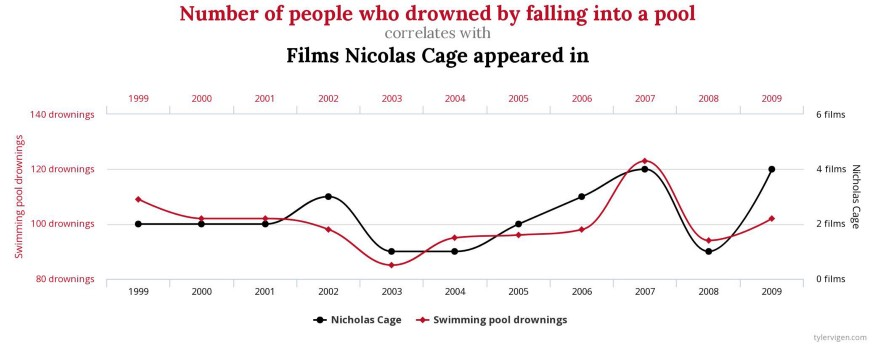
\includegraphics[width=0.5\textwidth]{Example_Data.jpeg}
\caption{\label{fig:rysunek_1}Przykładowy rysunek}
\end{figure}


\subsection{Część 2}
\begin{lstlisting}[language=Python]

import sys
#if
if __name__ == "__main__":

    def count_words():
        data = open(f'./{sys.argv[1]}')
        return_data = {}
        nums = data.read().split()
        distinct_nums = list(set(nums))
        for distinct_num in distinct_nums:
            return_data[distinct_num] = nums.count(distinct_num)

        data.close()
        return return_data

    if len(sys.argv) < 2:
        print('Za malo argumentow')
    elif len(sys.argv) > 2:
        print('Za duzo argumentow')
    else:
        counter_dict = count_words()
        count_words()
        f = open(f'./{sys.argv[1]}.par', "w+")
        f.write(f'Liczba roznych wyrazow: {len(counter_dict)}\n')
        f.write(str(counter_dict))
        f.close()

\end{lstlisting}

\pagebreak
\subsection{Część 3}

$$e=mc^2$$
$$\pi=\frac{c}{d}$$
$$\frac{d}{dx}e^x=e^x$$
$$\frac{d}{dx}\int_{0}^\infty f(s)ds = f(x)$$
$$f(x) = \sum_{i} = 0^\infty\frac{f^{(i)}(0)}{i!}x^i$$
$$x = \sqrt{\frac{x_i}{z}y}$$


\section{Zadanie 3}


\subsection{Część 1}
Wbrew pozorom, korelacja śmierci spowodowanych utonięciem w basenie\cite{saluja2006swimming} a wydawanymi filmami wydawanymi rocznie z określonym aktorem\cite{fearing1947influence} nie tworzy związku przyczynowego.


\subsection{Część 2}
\printbibliography


\end{document}
